% // TODO: Replace samples=40 por 200
\chapter{Splines}

In computer graphics, we often need to create smooth curves that can be easily manipulated. Curves have 3 different representations:
\begin{itemize}
    \item \ul{Explicit}: $y = f(x)$
    
    As a disadvantage, explicit curves cannot represent vertical lines, so they are not suitable for all types of curves.
    \item \ul{Implicit}: $f(x,y) = 0$
    
    As a disadvantage, implicit curves can be more difficult to work with, especially when it comes to rendering and manipulating them.
    \item \ul{Parametric}: $x = f(t), y = g(t)$
    
    Parametric curves are often preferred in computer graphics because they allow for more flexibility and control over the shape of the curve. They can represent a wider variety of curves, including those that cannot be represented in explicit form, such as vertical lines. Additionally, the problem is simplified, as we only consider one dimension at a time.
\end{itemize}

The main goal when working with curves is to interpolate some given points, which means finding a curve that passes through those points. Parametric curves are often used with the goal of interpolation, as they allow us to simply the problem by considering each coordinate separately, which is what we will do in the following sections. Some desired properties of the interpolating curve are:
\begin{itemize}
    \item \ul{$C^0$}: The curve is continuous, which means that there are no gaps or jumps in the curve.
    \item \ul{$C^1$}: A curve is parametric continuos $C^1$ if the curve is derivative continuous, which means that the curve has a well-defined tangent at every point, and there are no sharp corners or cusps in the curve.
    
    In each node, the curve is $C^1$ if the tangent of the curve is the same when approaching the node from the left and from the right.
    
    \item \ul{$G^1$}: A curve is geometric continuous $G^1$ if, at every node, the tangent of the curve has the same direction when approaching the node from the left and from the right, but it can have different magnitudes.
    \item \ul{$C^2$}: The curve is second derivative continuous, which means that the curve has a well-defined curvature at every point, and there are no inflection points.
\end{itemize}

Another important property of the curve is the \emph{Convex Hull Property}, which states that the curve is contained within the convex hull of its control points. Its control points are not only the points that we want to interpolate, but also the points that we use to define the shape of the curve. The convex hull of a set of points is the smallest convex shape that contains all of the points. The convex hull property is desirable because, when it is satisfied, in order to calculate intersections between the curve and other objects, we can first calculate the intersection between the convex hull and the other object, which is much easier to compute. If there is no intersection between the convex hull and the other object, then there is no intersection between the curve and the other object, so we can avoid performing more complex calculations. The needed and sufficient condition for a curve to satisfy the convex hull property is:
\begin{itemize}
    \item The curve is a linear combination of its control points, which means that the curve can be expressed as a weighted sum of its control points, where the weights are non-negative and sum up to 1.
    \begin{equation*}
        P(t) = \sum_{i=0}^{n} w_i(t) P_i
    \end{equation*}
    where:
    \begin{itemize}
        \item $\sum_{i=0}^{n} w_i(t) = 1$ for all $t$.
        \item $w_i(t) \geq 0$ for all $i$ and for all $t$.
    \end{itemize}
\end{itemize}


\section{Polinomial Interpolation}

Given a set of $n$ points, the aim is to find a polynomial of degree $n-1$ (which is the lowest degree possible) that passes through all of those points. The polynomial can be expressed as:
\[P(t) = \sum_{i=0}^{n-1} a_i t^i\]
where $a_i$ are the coefficients of the polynomial and $t^i$ are the monomials. There are different methods to find the coefficients $a_i$.

\subsection{Undetermined Coefficients}

This method involves setting up a system of equations based on the given points and solving for the coefficients $a_i$. For each point $(t_j, y_j)$, we can substitute it into the polynomial equation to get:
\[y_j = \sum_{i=0}^{n-1} a_i t_j^i\]
This results in a system of $n$ equations with $n$ unknowns (the coefficients $a_i$). We can solve this system using methods such as Gaussian elimination or matrix inversion.

\subsection{Lagrange Interpolation}

The Lagrange interpolation method constructs the polynomial using a linear combination of basis polynomials. The Lagrange basis polynomial for the $i$-th point is defined as:
\[L_i(t) = \prod_{j=0, j \neq i}^{n-1} \frac{t - t_j}{t_i - t_j}\]
These basis polynomials have the property that:
\[L_i(t_j) = \delta_{ij} = \begin{cases}1 & \text{if } i = j \\ 0 & \text{if } i \neq j\end{cases}\]
Therefore, the interpolating polynomial can be expressed as:
\[P(t) = \sum_{i=0}^{n-1} y_i L_i(t)\]
This method is straightforward and does not require solving a system of equations, but it can be computationally expensive for large $n$ due to the need to compute the basis polynomials.

\subsection{Runge's Phenomenon}

When using high-degree polynomials for interpolation, especially with equally spaced points, we can encounter Runge's phenomenon, which is characterized by large oscillations at the edges of the interval. In the Figure~\ref{fig:runge} we can see an example of this phenomenon, where the interpolating polynomial oscillates significantly, even though it passes through all the given points (being therefore a perfect fit). This is a major drawback of using high-degree polynomials for interpolation, and it motivates the use of alternative methods such as splines, which we will discuss in the next section.

\begin{figure}
    \centering
    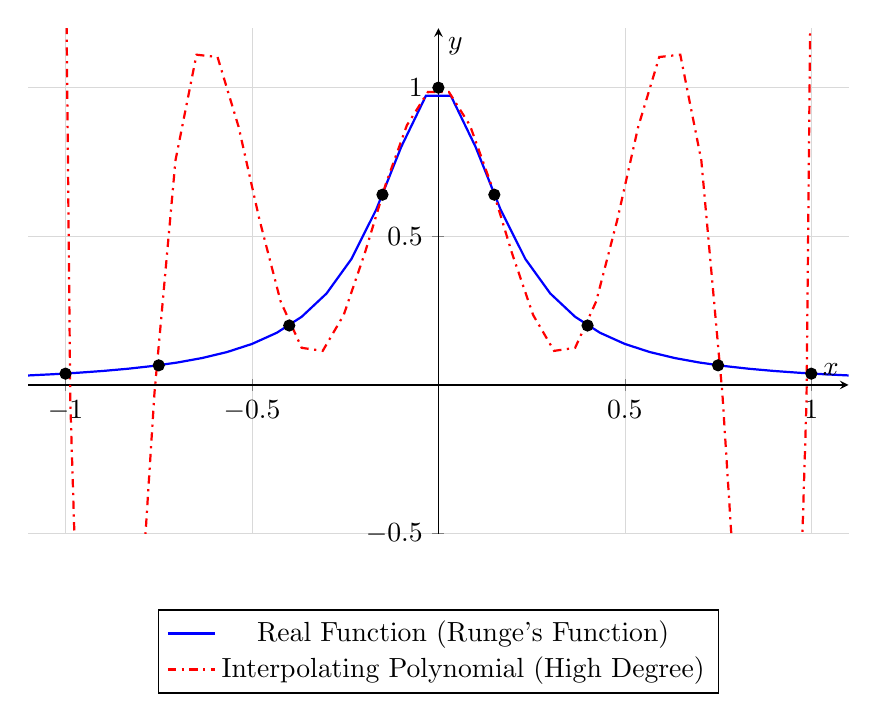
\begin{tikzpicture}
    \begin{axis}[
        width=12cm, height=8cm,
        xmin=-1.1, xmax=1.1,
        ymin=-0.5, ymax=1.2,
        axis lines=middle,
        xlabel={$x$}, ylabel={$y$},
        grid=both,
        grid style={line width=.1pt, draw=gray!10},
        major grid style={line width=.2pt, draw=gray!30},
        xtick={-1, -0.5, 0, 0.5, 1},
        ytick={-0.5, 0, 0.5, 1},
        samples=40,
        legend style={at={(0.5,-0.15)}, anchor=north},
    ]

        % 1. Función original de Runge: f(x) = 1 / (1 + 25x^2)
        \addplot[
            domain=-1.3:1.3, 
            thick, 
            blue
        ] {1 / (1 + 25*x^2)};
        \addlegendentry{Real Function (Runge's Function)}


        % 2. Polinomio interpolador oscilatorio (Simulación cualitativa de grado alto)
        % Usamos una aproximación polinómica que muestra las oscilaciones típicas en los bordes
        \addplot[
            domain=-1.1:1.1, 
            thick, 
            red, 
            dashdotted
        ] {128.68*x^8 - 227.9*x^6 + 117.8*x^4 - 18.54*x^2 + 1};
        \addlegendentry{Interpolating Polynomial (High Degree)}


        % 3. Nodos de interpolación (Puntos equiespaciados donde se cruzan)
        % Graficamos algunos puntos clave donde el polinomio toca a la función
        \addplot[
            only marks, 
            mark=*, 
            mark size=2pt, 
            black
        ] coordinates {
            (-1, 0.038) (-0.75, 0.066) (-0.4, 0.2) (-0.15, 0.64) (0, 1) 
            (0.15, 0.64) (0.4, 0.2) (0.75, 0.066) (1, 0.038)
        };

    \end{axis}
    \end{tikzpicture}
    \caption{Runge's Phenomenon}
    \label{fig:runge}
\end{figure}


\section{Splines}

To overcome the issues associated with high-degree polynomial interpolation, we can use splines. A spline is a piecewise polynomial function that is defined on a set of intervals, with each interval having its own polynomial. Therefore, when there is a lot of points to interpolate, a common practice is to divide the interval into different segments (when each segment contains two points) and use a low-degree polynomial to interpolate the points in each segment. After that, we can connect the segments together to form a smooth curve. This approach allows us to achieve a smooth curve without the oscillations associated with high-degree polynomials. During the following sections, we will discuss different types of splines and their properties.

\subsection{Constant Splines}

The simplest type of spline is the constant spline, which is a piecewise constant function. In each segment, the function takes the value of the starting point of the segment. Mathematically, it can be defined as:
\[S(t) = y_i \quad \text{for } t_i \leq t < t_{i+1}\]

An example of a constant spline is shown in the Figure~\ref{fig:constant_spline}. As we can see, the curve is not even continuous, as it has jumps at the knots, so more complex splines are usually preferred.
\begin{figure}
    \centering
    \begin{tikzpicture}
    \begin{axis}[
        width=12cm, height=8cm,
        xmin=-0.5, xmax=4.5,
        ymin=-0.5, ymax=1.5,
        axis lines=middle,
        xlabel={$t$}, ylabel={$S(t)$},
        grid=both,
        grid style={line width=.1pt, draw=gray!10},
        major grid style={line width=.2pt, draw=gray!30},
        xtick={0, 1, 2, 3, 4},
        ytick={0, 0.5, 1},
        samples=40,
    ]

        % Interpolating points
        \addplot[
            only marks, 
            mark=*, 
            mark size=2pt, 
            black
        ] coordinates {
            (0, 1) (1, 0.5) (2, 1) (3, 0) (4, 1)
        };

        % Constant spline segments
        \addplot[
            domain=0:1,
            thick,
            blue
        ] {1};
        \addplot[
            domain=1:2,
            thick,
            blue
        ] {0.5};
        \addplot[
            domain=2:3,
            thick,
            blue
        ] {1};
        \addplot[
            domain=3:4,
            thick,
            blue
        ] {0};
        \addplot[
            domain=4:4.5,
            thick,
            blue
        ] {1};
        
    \end{axis}
    \end{tikzpicture}
    \caption{Constant Spline Example}
    \label{fig:constant_spline}
\end{figure}


\subsection{Linear Splines}

A linear spline is a piecewise linear function that connects the given points with straight lines. In each segment, the function is defined as the linear interpolation between the two points that define the segment. Mathematically, it is defined as:
\[S(t) = y_i + \frac{y_{i+1} - y_i}{t_{i+1} - t_i} (t - t_i) \quad \text{for } t_i \leq t < t_{i+1}\]
An example of a linear spline is shown in the Figure~\ref{fig:linear_spline}. As we can see, the curve is continuous, but it is not smooth, as it has sharp corners at the knots. This is why we usually prefer to use cubic splines, which we will discuss in the next section.
\begin{figure}
    \centering
    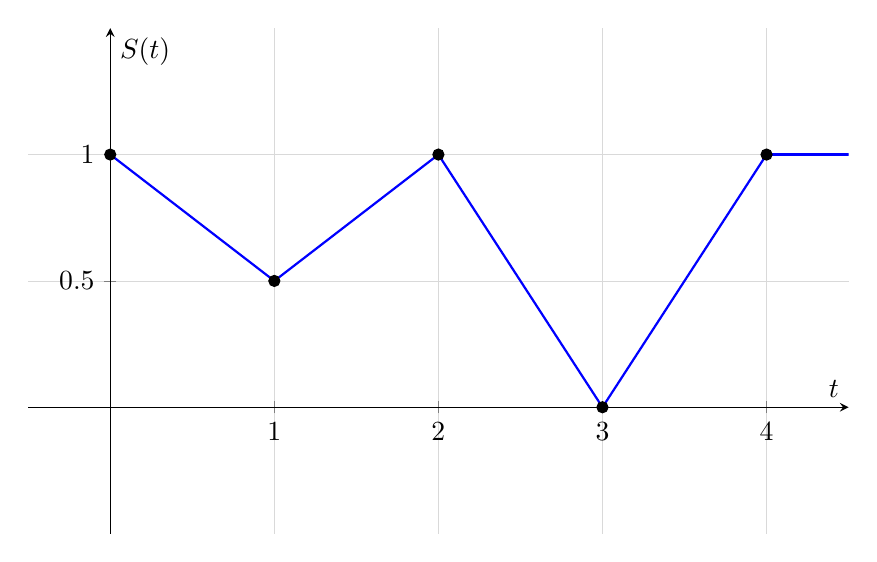
\begin{tikzpicture}
    \begin{axis}[
        width=12cm, height=8cm,
        xmin=-0.5, xmax=4.5,
        ymin=-0.5, ymax=1.5,
        axis lines=middle,
        xlabel={$t$}, ylabel={$S(t)$},
        grid=both,
        grid style={line width=.1pt, draw=gray!10},
        major grid style={line width=.2pt, draw=gray!30},
        xtick={0, 1, 2, 3, 4},
        ytick={0, 0.5, 1},
        samples=2,
    ]

        % Interpolating points
        \addplot[
            only marks, 
            mark=*, 
            mark size=2pt, 
            black
        ] coordinates {
            (0, 1) (1, 0.5) (2, 1) (3, 0) (4, 1)
        };

        % Linear spline segments
        \addplot[
            domain=0:1,
            thick,
            blue
        ] {1 - 0.5*x};
        \addplot[
            domain=1:2,
            thick,
            blue
        ] {0.5 + 0.5*(x-1)};
        \addplot[
            domain=2:3,
            thick,
            blue
        ] {1 - x + 2};
        \addplot[
            domain=3:4,
            thick,
            blue
        ] {0 + x - 3};
        \addplot[
            domain=4:4.5,
            thick,
            blue
        ] {1};

    \end{axis}
    \end{tikzpicture}
    \caption{Linear Spline Example}
    \label{fig:linear_spline}
\end{figure}

During the following sections, we will discuss different types of cubic splines. They are the most commonly used type of splines, as they provide a good balance between smoothness and computational efficiency. Without loss of generality, we will consider the interval $t\in [0,1]$. In each segment, the function is defined as a cubic polynomial that interpolates the two points that define the segment. However, a third degree polynomial has 4 coefficients, so we need to impose 2 additional conditions to be able to solve for those coefficients. Different types of cubic splines are defined based on the additional conditions that we impose.

\subsection{Hermite Cubic Splines}

\begin{observacion}
    \myhref{https://www.geogebra.org/m/qcnrgnbg}{This interactive applet} shows how the Hermite splines work, and will help the user to understand this concept.
\end{observacion}

A Hermite cubic spline is a piecewise cubic function that is defined by the values of the function and its derivative at the endpoints of each segment. In other words, if the interpolating polynomial is $P$, we have the following conditions:
\begin{align*}
    P(0) &= y_0 \\
    P(1) &= y_1 \\
    P'(0) &= m_0 \\
    P'(1) &= m_1
\end{align*}
where $y_0$ and $y_1$ are the values of the function at the endpoints of the segment, and $m_0$ and $m_1$ are the values of the derivative\footnote{The corresponding coordinate of the derivative, as we are working with parametric equations.} at the endpoints of the segment. After solving and rearranging the equations, we can express the Hermite cubic spline as:
\begin{align*}
    P(t) &= H_{y_0}(t) y_0 + H_{y_1}(t) y_1 + H_{m_0}(t) m_0 + H_{m_1}(t) m_1
\end{align*}
where $H_{y_0}(t)$, $H_{y_1}(t)$, $H_{m_0}(t)$ and $H_{m_1}(t)$ are the Hermite basis functions, shown in Figure~\ref{fig:hermite_basis} and defined as:
\begin{align*}
    H_{y_0}(t) &=  (1 - t)^2(1 + 2t) \\
    H_{y_1}(t) &= (3 - 2t)t^2 \\
    H_{m_0}(t) &= t(1 - t)^2 \\
    H_{m_1}(t) &= t^2 (t - 1)
\end{align*}
\begin{figure}
    \centering
    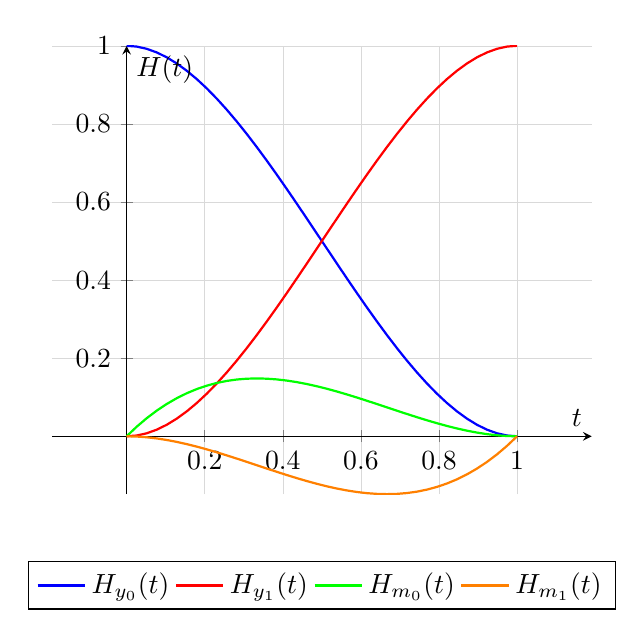
\begin{tikzpicture}
    \begin{axis}[
        axis equal,
        axis lines=middle,
        xlabel={$t$}, ylabel={$H(t)$},
        grid=both,
        grid style={line width=.1pt, draw=gray!10},
        major grid style={line width=.2pt, draw=gray!30},
        samples=40,
        legend style={at={(0.5,-0.15)}, anchor=north, legend columns=4},
    ]

        % Hermite basis functions
        \addplot[
            domain=0:1,
            thick,
            blue
        ] {(1 - x)^2 * (1 + 2*x)};
        \addlegendentry{$H_{y_0}(t)$}

        \addplot[
            domain=0:1,
            thick,
            red
        ] {(3 - 2*x)*x^2};
        \addlegendentry{$H_{y_1}(t)$}

        \addplot[
            domain=0:1,
            thick,
            green
        ] {x*(1 - x)^2};
        \addlegendentry{$H_{m_0}(t)$}

        \addplot[
            domain=0:1,
            thick,
            orange
        ] {x^2 * (x - 1)};
        \addlegendentry{$H_{m_1}(t)$}

    \end{axis}
    \end{tikzpicture}
    \caption{Hermite Basis Functions}
    \label{fig:hermite_basis}
\end{figure}
\begin{proof}
    A general cubic polynomial can be expressed as:
    \[P(t) = \sum_{i=0}^{3} a_i t^i
    = \begin{pmatrix}
        1 & t & t^2 & t^3
    \end{pmatrix}
    \begin{pmatrix}
        a_0 \\ a_1 \\ a_2 \\ a_3
    \end{pmatrix}\]

    Our aim is to find the coefficients $a_i$ such that the conditions of the Hermite cubic spline are satisfied. We can express the conditions in matrix form as:
    \[\begin{pmatrix}
    1 & 0 & 0 & 0 \\
    1 & 1 & 1 & 1 \\
    0 & 1 & 0 & 0 \\
    0 & 1 & 2 & 3
    \end{pmatrix}
    \begin{pmatrix}
        a_0 \\ a_1 \\ a_2 \\ a_3
    \end{pmatrix} =
    \begin{pmatrix}
        y_0 \\ y_1 \\ m_0 \\ m_1
    \end{pmatrix}\]

    We can solve this system of equations to find the coefficients $a_i$. Inverting the matrix on the left-hand side, we get:
    \[\begin{pmatrix}
    1 & 0 & 0 & 0 \\
    0 & 0 & 0 & 1 \\
    -3 & 3 & -2 & -1 \\
    2 & -2 & 1 & 1
    \end{pmatrix}
    \begin{pmatrix}
        y_0 \\ y_1 \\ m_0 \\ m_1
    \end{pmatrix} =
    \begin{pmatrix}
        a_0 \\ a_1 \\ a_2 \\ a_3
    \end{pmatrix}\]

    Therefore, the polynomial can be expressed as:
    \[P(t) =
    \begin{pmatrix}
        1 & t & t^2 & t^3
    \end{pmatrix}
    \begin{pmatrix}
    1 & 0 & 0 & 0 \\
    0 & 0 & 0 & 1 \\
    -3 & 3 & -2 & -1 \\
    2 & -2 & 1 & 1
    \end{pmatrix}
    \begin{pmatrix}
        y_0 \\ y_1 \\ m_0 \\ m_1
    \end{pmatrix}\]

    Multiplying the first two matrices, we get:
    \[P(t) =
    \begin{pmatrix}
    H_{y_0}(t) & H_{y_1}(t) & H_{m_0}(t) & H_{m_1}(t)
    \end{pmatrix}
    \begin{pmatrix}
        y_0 \\ y_1 \\ m_0 \\ m_1
    \end{pmatrix}\]
    where $H_{y_0}(t)$, $H_{y_1}(t)$, $H_{m_0}(t)$ and $H_{m_1}(t)$ are the Hermite basis functions presented above.
\end{proof}

Once each segment is defined, we can connect them together imposing $C^1$ continuity at the knots, which means that the derivative of the curve is continuous at the knots. This type of spline has however some disadvantages:
\begin{itemize}
    \item It does not satisfy the convex hull property, as the basis functions can take negative values.
    \item It is not only controlled by points but also by the derivatives at the endpoints of each segment (vectors). This has several disadvantages:
    \begin{itemize}
        \item It is not intuitive to control the shape of the curve by manipulating the derivatives at the endpoints of each segment.
        \item It requires special care when transforming the curve. Points can always be transformed using the same transformation, but vectors need to be transformed using the inverse transpose of the transformation, which can be more complex to implement.
    \end{itemize}
\end{itemize}

\subsubsection{Catmull-Rom Splines}

Hermite cubic splines require us to specify the derivative at the endpoints of each segment, which can be difficult to control. A common practice is to use the Catmull-Rom spline, which is a type of Hermite cubic spline where the derivative at each node is defined as:
\begin{align*}
    m_0 &= y_1 - y_0 \\
    m_i &= \frac{(y_{i+1} - y_i) + (y_i - y_{i-1})}{2} = \frac{y_{i+1} - y_{i-1}}{2} \quad \text{for } i = 1, \ldots, n-1 \\
    m_{n} &= y_{n} - y_{n-1}
\end{align*}

It should be noted that it simply defines the derivative at each node as the average of the slopes of the segments that connect the node to its neighbors, which is a simple and intuitive way to control the shape of the curve.


\subsection{Bezier Cubic Splines}
\begin{observacion}
    \myhref{https://www.geogebra.org/m/qcnrgnbg}{This interactive applet} shows how the Bezier splines work, and will help the user to understand this concept.
\end{observacion}
A Bezier cubic spline is a piecewise cubic function that is defined by four control points: the two endpoints of the segment and two additional control points that determine the shape of the curve. The conditions for a Bezier cubic spline are:
\begin{align*}
    P(0) &= y_0 \\
    P(1) &= y_3 \\
    P'(0) &= 3(y_1 - y_0) \\
    P'(1) &= 3(y_3 - y_2)
\end{align*}
where $y_0$ and $y_3$ are the endpoints of the segment, and $y_1$ and $y_2$ are the control points that determine the shape of the curve. The two additional conditions simply represent the derivative\footnote{It should be noted that, in fact, it is not the derivate but its equivalent in only one dimension.} of the curve at the endpoints (scaled by 3), which is determined by the control points. After solving and rearranging the equations, we can express the Bezier cubic spline as:
% // TODO: Por qué se escala por 3?
\begin{align*}
    P(t) &= B_{y_0}(t) y_0 + B_{y_1}(t) y_1 + B_{y_2}(t) y_2 + B_{y_3}(t) y_3
\end{align*}
where $B_{y_0}(t)$, $B_{y_1}(t)$, $B_{y_2}(t)$ and $B_{y_3}(t)$ are the Bezier basis functions, shown in Figure~\ref{fig:bezier_basis} and defined as:
\begin{align*}
    B_{y_0}(t) &= (1 - t)^3 \\
    B_{y_1}(t) &= 3t(1 - t)^2 \\
    B_{y_2}(t) &= 3t^2(1 - t) \\
    B_{y_3}(t) &= t^3
\end{align*}

In general, the Bezier basic functions can be defined for any degree $n$ as:
\begin{align*}
    B_{y_i}(t) &= \binom{n}{i} t^i (1 - t)^{n - i}
\end{align*}
\begin{figure}
    \centering
    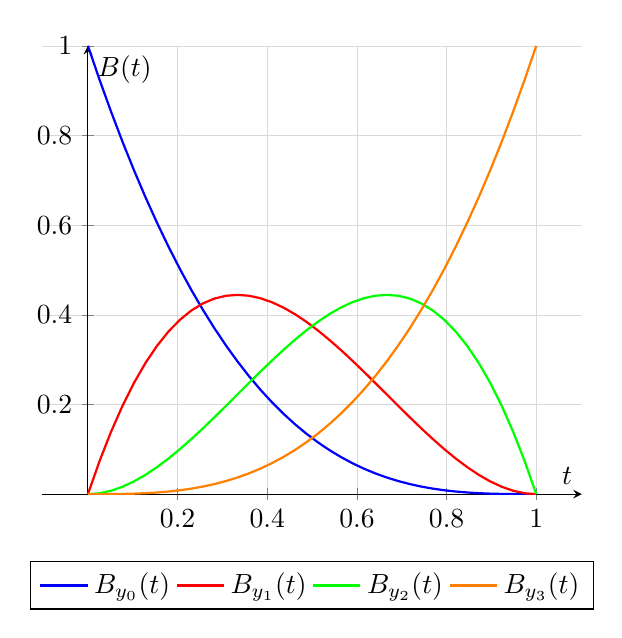
\begin{tikzpicture}
    \begin{axis}[
        axis equal,
        axis lines=middle,
        xlabel={$t$}, ylabel={$B(t)$},
        grid=both,
        grid style={line width=.1pt, draw=gray!10},
        major grid style={line width=.2pt, draw=gray!30},
        samples=40,
        legend style={at={(0.5,-0.15)}, anchor=north, legend columns=4},
    ]

        % Bezier basis functions
        \addplot[
            domain=0:1,
            thick,
            blue
        ] {(1 - x)^3};
        \addlegendentry{$B_{y_0}(t)$}

        \addplot[
            domain=0:1,
            thick,
            red
        ] {3*x*(1 - x)^2};
        \addlegendentry{$B_{y_1}(t)$}

        \addplot[
            domain=0:1,
            thick,
            green
        ] {3*x^2*(1 - x)};
        \addlegendentry{$B_{y_2}(t)$}

        \addplot[
            domain=0:1,
            thick,
            orange
        ] {x^3};
        \addlegendentry{$B_{y_3}(t)$}

    \end{axis}
    \end{tikzpicture}
    \caption{Bezier Basis Functions}
    \label{fig:bezier_basis}
\end{figure}
\begin{proof}
    A general cubic polynomial can be expressed as:
    \[P(t) = \sum_{i=0}^{3} a_i t^i
    = \begin{pmatrix}
        1 & t & t^2 & t^3
    \end{pmatrix}
    \begin{pmatrix}
        a_0 \\ a_1 \\ a_2 \\ a_3
    \end{pmatrix}\]

    Our aim is to find the coefficients $a_i$ such that the conditions of the Bezier cubic spline are satisfied.
    \begin{align*}
        P(0) &= a_0 = y_0 \\
        P(1) &= a_0 + a_1 + a_2 + a_3 = y_3 \\
        P'(0) &= a_1 = 3y_1 - 3y_0 \\
        P'(1) &= a_1 + 2a_2 + 3a_3 = 3y_3 - 3y_2
    \end{align*}

    Rearranging the equations and expressing them in matrix form, we get:
    \[\begin{pmatrix}
    1 & 0 & 0 & 0 \\
    1 & \nicefrac{1}{3} & 0 & 0 \\
    1 & \nicefrac{2}{3} & \nicefrac{1}{3} & 0 \\
    1 & 1 & 1 & 1
    \end{pmatrix}
    \begin{pmatrix}
        a_0 \\ a_1 \\ a_2 \\ a_3
    \end{pmatrix} =
    \begin{pmatrix}
        y_0 \\ y_1 \\ y_2 \\ y_3
    \end{pmatrix}\]

    Inverting the matrix on the left-hand side, we get:
    \[\begin{pmatrix}
    1 & 0 & 0 & 0 \\
    -3 & 3 & 0 & 0 \\
    3 & -6 & 3 & 0 \\
    -1 & 3 & -3 & 1
    \end{pmatrix}
    \begin{pmatrix}
        y_0 \\ y_1 \\ y_2 \\ y_3
    \end{pmatrix} =
    \begin{pmatrix}
        a_0 \\ a_1 \\ a_2 \\ a_3
    \end{pmatrix}\]

    Therefore, the polynomial can be expressed as:
    \[P(t) =
    \begin{pmatrix}
        1 & t & t^2 & t^3
    \end{pmatrix}
    \begin{pmatrix}
    1 & 0 & 0 & 0 \\
    -3 & 3 & 0 & 0 \\
    3 & -6 & 3 & 0 \\
    -1 & 3 & -3 & 1
    \end{pmatrix}
    \begin{pmatrix}
        y_0 \\ y_1 \\ y_2 \\ y_3
    \end{pmatrix}\]
    
    Multiplying the first two matrices, we get:
    \[P(t) =
    \begin{pmatrix}
    B_{y_0}(t) & B_{y_1}(t) & B_{y_2}(t) & B_{y_3}(t)
    \end{pmatrix}
    \begin{pmatrix}
        y_0 \\ y_1 \\ y_2 \\ y_3
    \end{pmatrix}\]
    where $B_{y_0}(t)$, $B_{y_1}(t)$, $B_{y_2}(t)$ and $B_{y_3}(t)$ are the Bezier basis functions presented above.
\end{proof}

Once each segment is defined, we can connect them together imposing $C^0$ continuity at the knots. Some specific characteristics of Bezier cubic splines are:
\begin{itemize}
    \item They do satisfy the convex hull property (as the basis functions are non-negative and sum up to 1).
    \item They are only controlled by points, which is more intuitive than controlling the shape of the curve by manipulating the derivatives at the endpoints of each segment, as in Hermite cubic splines.
    \item They do not require special care when transforming the curve, as all the control points can be transformed using the same transformation, unlike in Hermite cubic splines where we need to transform points and vectors differently.
    \item For each knot, if its previous and next control points are collinear with the knot, then the curve is $G^1$ continuous at that knot, as the tangent of the curve has the same direction when approaching the knot from the left and from the right.
\end{itemize}

\subsubsection{De Casteljau's Algorithm}

De Casteljau's algorithm is a recursive method for evaluating Bezier curves at a given parameter value $t$. It is based on the principle of linear interpolation and can be used to compute points on the Bezier curve efficiently, and can also be used to graphically represent the curve. Let's see an example of how De Casteljau's algorithm works for a cubic Bezier curve defined by control points $y_0$, $y_1$, $y_2$ and $y_3$.
\begin{align*}
    P(t) &= B_{y_0}(t) y_0 + B_{y_1}(t) y_1 + B_{y_2}(t) y_2 + B_{y_3}(t) y_3 \\
    &= (1 - t)^3 y_0 + 3t(1 - t)^2 y_1 + 3t^2(1 - t) y_2 + t^3 y_3
    \\&= (1 - t) \left\{ (1 - t)\left[ (1 - t) y_0 + t y_1 \right] + t \left[ (1 - t) y_1 + t y_2 \right] \right\} +\\&\hspace{1.1cm}+ t \left\{ (1 - t) \left[ (1 - t) y_1 + t y_2 \right] + t \left[ (1 - t) y_2 + t y_3 \right] \right\}
\end{align*}

As we can see, several interpolations are made:
\begin{itemize}
    \item First, we interpolate between the control points to get three new points:
    \begin{align*}
        y_{01} &= (1 - t) y_0 + t y_1 \\
        y_{12} &= (1 - t) y_1 + t y_2 \\
        y_{23} &= (1 - t) y_2 + t y_3
    \end{align*}
    where $y_{ij}$ represents the point obtained by interpolating between the control points $y_i$ and $y_j$. It should be noted that $y_{12}$ is obtained twice.
    \item Then, we interpolate between the new points to get two new points:
    \begin{align*}
        y_{(01)(12)} &= (1 - t) y_{01} + t y_{12} \\
        y_{(12)(23)} &= (1 - t) y_{12} + t y_{23}
    \end{align*}
    \item Finally, we interpolate between the last two points to get the point on the curve corresponding to the parameter value $t$:
    \begin{align*}
        P(t) &= (1 - t) y_{(01)(12)} + t y_{(12)(23)}
    \end{align*}
\end{itemize}

Doing this process several times for different values of $t$ allows us to compute multiple points on the curve, which can be used to graphically represent the curve.


\subsection{B-Spline Cubic Splines}

Hermite and Bezier cubic splines have some disadvantages, such as not being able to achieve $C^2$ continuity at the knots. B-spline cubic splines address this issue but resign an important property: they do not interpolate the control points, but only approximate them. A B-spline cubic spline is a piecewise cubic function that is defined by a set of control points. In order to achieve $C^2$ continuity, the perspective is not to define the curve by independent segments, but by segments \emph{whose control points overlap}. The polynomial that defines the $i$-th segment is:
\begin{align*}
    P_i(t) &= \sum_{k=0}^{3} y_{i+k} B_k(t)
\end{align*}
where $y_{i+k}$ are the control points and $B_k(t)$ are the B-spline basis functions, shown in Figure~\ref{fig:bspline_basis} and defined as:
\begin{align*}
    B_0(t) &= \nicefrac{1}{6}\cdot (1 - t)^3 \\
    B_1(t) &= \nicefrac{1}{6}\cdot (3t^3 - 6t^2 + 4) \\
    B_2(t) &= \nicefrac{1}{6}\cdot (-3t^3 + 3 t^2 + 3t + 1) \\
    B_3(t) &= \nicefrac{1}{6}\cdot t^3
\end{align*}
\begin{figure}
    \centering
    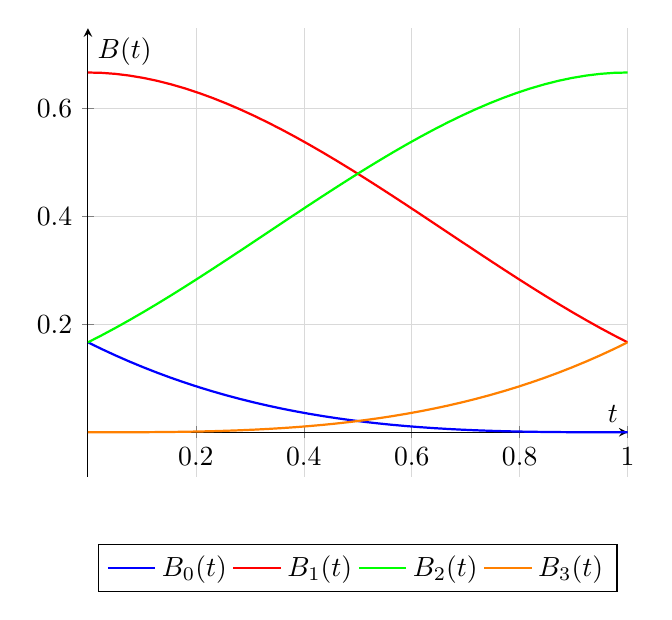
\begin{tikzpicture}
    \begin{axis}[
        axis equal,
        axis lines=middle,
        xlabel={$t$}, ylabel={$B(t)$},
        grid=both,
        grid style={line width=.1pt, draw=gray!10},
        major grid style={line width=.2pt, draw=gray!30},
        samples=40,
        legend style={at={(0.5,-0.15)}, anchor=north, legend columns=4},
    ]

        % B-spline basis functions
        \addplot[
            domain=0:1,
            thick,
            blue
        ] {(1 - x)^3 / 6};
        \addlegendentry{$B_0(t)$}

        \addplot[
            domain=0:1,
            thick,
            red
        ] {(3*x^3 - 6*x^2 + 4) / 6};
        \addlegendentry{$B_1(t)$}

        \addplot[
            domain=0:1,
            thick,
            green
        ] {(-3*x^3 + 3*x^2 + 3*x + 1) / 6};
        \addlegendentry{$B_2(t)$}

        \addplot[
            domain=0:1,
            thick,
            orange
        ] {x^3 / 6};
        \addlegendentry{$B_3(t)$}

    \end{axis}
    \end{tikzpicture}
    \caption{B-spline Basis Functions}
    \label{fig:bspline_basis}
\end{figure}

By the definition, it is perfectly clear that the control points of each segment overlap with the control points of the previous and next segments, as:
\begin{itemize}
    \item During the $i$-th segment, the control points are $y_i$, $y_{i+1}$, $y_{i+2}$ and $y_{i+3}$.
    \item During the $(i+1)$-th segment, the control points are $y_{i+1}$, $y_{i+2}$, $y_{i+3}$ and $y_{i+4}$. Three of the control points are shared with the previous segment, which allows us to achieve $C^2$ continuity.
    \item It should also be taken into account that $n$ control points define $n-3$ segments, as the $i$-th segment uses up to the $i+3$-th control point.
\end{itemize}

Let's adress know how to get to the basis functions. The conditions imposed to the B-spline cubic spline are:
\begin{itemize}
    \item $C^0$ continuity.
    
    That implies $P_i(1) = P_{i+1}(0)$ for all $i$. Therefore, we have:
    \begin{align*}
        \sum_{k=0}^{3} y_{i+k} B_k(1) &= \sum_{k=0}^{3} y_{i+1+k} B_k(0)
    \end{align*}

    Since that should be valid for every possible $y_j$ values, the conditions should be on the basis functions. Therefore, we have:
    \begin{align*}
        B_0(1) &= 0 \\
        B_1(1) &= B_0(0) \\
        B_2(1) &= B_1(0) \\
        B_3(1) &= B_2(0) \\
        B_3(0) &= 0
    \end{align*}

    \item $C^1$ continuity.
    
    That implies $P_i'(1) = P_{i+1}'(0)$ for all $i$. Therefore, we have:
    \begin{align*}
        \sum_{k=0}^{3} y_{i+k} B_k'(1) &= \sum_{k=0}^{3} y_{i+1+k} B_k'(0)
    \end{align*}

    As before, the conditions are:
    \begin{align*}
        B_0'(1) &= 0 \\
        B_1'(1) &= B_0'(0) \\
        B_2'(1) &= B_1'(0) \\
        B_3'(1) &= B_2'(0) \\
        B_3'(0) &= 0
    \end{align*}

    \item $C^2$ continuity.
    
    That implies $P_i''(1) = P_{i+1}''(0)$ for all $i$. Therefore, we have:
    \begin{align*}
        \sum_{k=0}^{3} y_{i+k} B_k''(1) &= \sum_{k=0}^{3} y_{i+1+k} B_k''(0)
    \end{align*}

    \item Up to this point, we have $5\cdot 3 = 15$ conditions. Since we have 4 basis functions each defined by a cubic polynomial, we have $4\cdot 4 = 16$ coefficients to determine, so we need one more condition.
    
    In order to have the convex hull property, we need the basis functions to be non-negative and sum up to 1. Therefore, the last condition is:
    \begin{align*}
        B_0(0) + B_1(0) + B_2(0) + B_3(0) &= 1
    \end{align*}
\end{itemize}

After solving the system of equations defined by the conditions above, we get the basis functions presented at the beginning of this section. Given the conditions that are imposed to the B-spline cubic spline, it is not surprising that the basis functions match in a very speciall way, shown in Figure~\ref{fig:bspline_basis_match}.
\begin{figure}
    \centering
    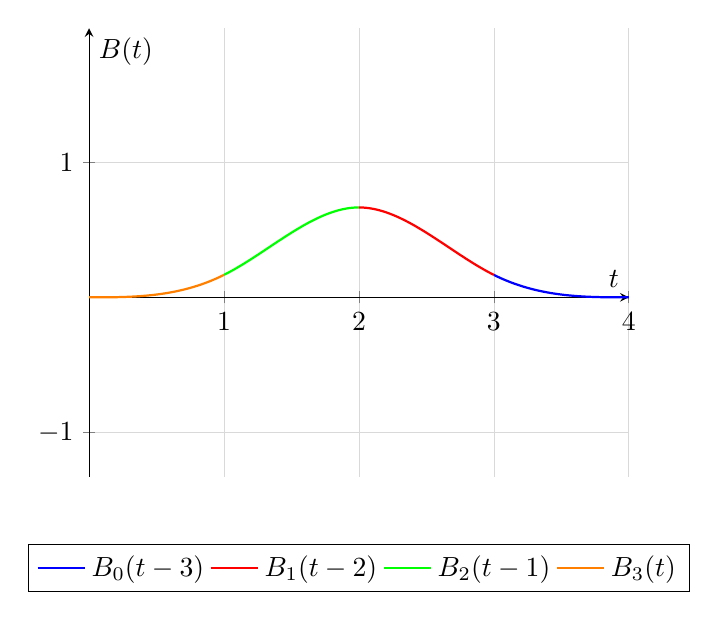
\begin{tikzpicture}
    \begin{axis}[
        axis equal,
        axis lines=middle,
        xlabel={$t$}, ylabel={$B(t)$},
        grid=both,
        grid style={line width=.1pt, draw=gray!10},
        major grid style={line width=.2pt, draw=gray!30},
        samples=40,
        legend style={at={(0.5,-0.15)}, anchor=north, legend columns=4},
    ]

        % B-spline basis functions
        \addplot[
            domain=3:4,
            thick,
            blue
        ] {(1 - (x - 3))^3 / 6};
        \addlegendentry{$B_0(t-3)$}
        \addplot[
            domain=2:3,
            thick,
            red
        ] {(3*(x - 2)^3 - 6*(x - 2)^2 + 4) / 6};
        \addlegendentry{$B_1(t-2)$}
        \addplot[
            domain=1:2,
            thick,
            green
        ] {(-3*(x - 1)^3 + 3*(x - 1)^2 + 3*(x - 1) + 1) / 6};
        \addlegendentry{$B_2(t-1)$}
        \addplot[
            domain=0:1,
            thick,
            orange
        ] {(x)^3 / 6};
        \addlegendentry{$B_3(t)$}
    \end{axis}
    \end{tikzpicture}
    \caption{B-spline Basis Functions Match}
    \label{fig:bspline_basis_match}
\end{figure}

Even though B-spline cubic splines do not interpolate the control points, they have some advantages:
\begin{itemize}
    \item They do satisfy the convex hull property, as the basis functions are non-negative and sum up to 1.
    \item They are only controlled by points, which is more intuitive than controlling the shape of the curve by manipulating the derivatives at the endpoints of each segment, as in Hermite cubic splines.
    \item They do not require special care when transforming the curve, as all the control points can be transformed using the same transformation, unlike in Hermite cubic splines where we need to transform points and vectors differently.
    \item They achieve $C^2$ continuity at the knots, which is not possible with Hermite and Bezier cubic splines.
\end{itemize}

\subsubsection{Achieving Interpolation with B-spline Cubic Splines}

Even though B-spline cubic splines do not interpolate the control points, we can achieve interpolating a point by repeating it three times.
Since in each segment, we have 4 control points:
\begin{itemize}
    \item If the segments where the first three control points are the same, then the curve will start in that point.
    \item If the segments where the last three control points are the same, then the curve will end in that point.
\end{itemize}

Therefore, the different situations are:
\begin{itemize}
    \item If we want to interpolate the first point, we need to repeat it three times at the beginning of the control points list, and the first segment will start in that point.
    \item If we want to interpolate the last point, we need to repeat it three times at the end of the control points list, and the last segment will end in that point.
    \item If we want to interpolate a point in the middle, we need to repeat it three times in the middle of the control points list, and a segment will end in that point and the next segment will start in that point.
\end{itemize}


\section{Parametric Surfaces}

Even though splines are commonly used to represent curves, they can also be used to represent surfaces. A parametric surface is a function that maps a pair of parameters $(u,v)$ to a point in 3D space. Space is divided into patches, and each patch is defined by a parametric function. In each patch, a total of $n\cdot m$ control points are used, where:
\begin{itemize}
    \item $n$ is the number of control points in the $u$ direction.
    \item $m$ is the number of control points in the $v$ direction.
\end{itemize}

After creating a grid-like structure with the control points, when interpolating a point on the surface with parameters $(u,v)$, the process is as follows (shown in Figure~\ref{fig:parametric_surface_interpolation}):
\begin{figure}
    \centering
    \begin{tikzpicture}[x=1cm, y=1cm, -Stealth, scale=1.0]

        % ====================================================================
        % PASO 1: Red Original de Puntos de Control
        % ====================================================================
        \begin{scope}[shift={(0,0)}]
            \node[anchor=south west, font=\bfseries\sffamily\small] at (-0.5, 3.8) {1: Place $P_{i,j}$ in a grid};
            
            % Definición de coordenadas para la malla
            \foreach \i/\y in {1/3, 2/2, 3/1, 4/0} {
                \foreach \j/\x in {1/0, 2/1, 3/2, 4/3} {
                    \pgfmathsetmacro{\xcoord}{\x + 0.25*\y}
                    \pgfmathsetmacro{\ycoord}{\y + 0.15*\x}
                    \coordinate (P\i\j) at (\xcoord,\ycoord);
                    \node[anchor=south, font=\tiny] at (P\i\j) {$P_{\i\j}$};
                }
            }
            
            % Dibujar las líneas de la malla
            \foreach \i in {1,2,3,4} {
                \draw[gray!40, dashed, thick] (P\i1) -- (P\i2) -- (P\i3) -- (P\i4);
            }
            \foreach \j in {1,2,3,4} {
                \draw[gray!40, dashed, thick] (P1\j) -- (P2\j) -- (P3\j) -- (P4\j);
            }
            
            % Dibujar los nodos
            \foreach \i in {1,2,3,4} {
                \foreach \j in {1,2,3,4} {
                    \fill[draw=black, fill=white, thick] (P\i\j) circle (2pt);
                }
            }
            
            % Etiquetas de las direcciones
            \draw[-Stealth, thick, blue] (-0.4,-0.4) -- (0.8,-0.2) node[midway, below, sloped, font=\tiny] {Dir $v$ ($j$)};
            \draw[-Stealth, thick, red] (-0.4,-0.4) -- (-0.2,0.8) node[midway, left, font=\tiny] {Dir $u$ ($i$)};
        \end{scope}

        % Flecha de transición 1
        \draw[-Stealth, ultra thick, gray!60] (4.2, 1.8) -- (4.9, 1.8);

        % ====================================================================
        % PASO 2: Curvas intermedias fijando 'v' (Cálculo de P_i(v))
        % ====================================================================
        \begin{scope}[shift={(5.2,0)}]
            \node[anchor=south west, font=\bfseries\sffamily\small] at (0.0, 3.8) {2: Interpolation in $v$};
            
            \foreach \i/\y in {1/3, 2/2, 3/1, 4/0} {
                \foreach \j/\x in {1/0, 2/1, 3/2, 4/3} {
                    \pgfmathsetmacro{\xcoord}{\x + 0.25*\y}
                    \pgfmathsetmacro{\ycoord}{\y + 0.15*\x}
                    \coordinate (Q\i\j) at (\xcoord,\ycoord);
                }
            }
            
            % Fondo atenuado
            \foreach \i in {1,2,3,4} { \draw[gray!20, dashed] (Q\i1) -- (Q\i4); }
            \foreach \j in {1,2,3,4} { \draw[gray!20, dashed] (Q1\j) -- (Q4\j); }
            \foreach \i in {1,2,3,4} { \foreach \j in {1,2,3,4} { \fill[gray!30] (Q\i\j) circle (1.5pt); } }
            
            % Curvas interpoladas en v
            \draw[blue!60, thick] (Q11) .. controls ($(Q11)+(0.6,0.2)$) and ($(Q14)-(0.6,0.2)$) .. (Q14);
            \draw[blue!60, thick] (Q21) .. controls ($(Q21)+0.6*(0.2,0.15)$) and ($(Q24)-0.6*(0.2,0.15)$) .. (Q24);
            \draw[blue!60, thick] (Q31) .. controls ($(Q31)+0.6*(0.2,0.1)$) and ($(Q34)-0.6*(0.2,0.1)$) .. (Q34);
            \draw[blue!60, thick] (Q41) .. controls ($(Q41)+0.6*(0.2,0.05)$) and ($(Q44)-0.6*(0.2,0.05)$) .. (Q44);
            
            % Puntos intermedios evaluados para un v fijo
            \coordinate (Pi1) at ($(Q11)!0.45!(Q14)+(0.05,0.1)$);
            \coordinate (Pi2) at ($(Q21)!0.45!(Q24)+(0.03,0.06)$);
            \coordinate (Pi3) at ($(Q31)!0.45!(Q34)+(0.01,0.03)$);
            \coordinate (Pi4) at ($(Q41)!0.45!(Q44)+(0.0,0.0)$);
            
            \draw[red!40, dashed, thick] (Pi1) -- (Pi2) -- (Pi3) -- (Pi4);
            
            \fill[blue] (Pi1) circle (2.5pt) node[right=1pt, font=\tiny] {$P_0(v)$};
            \fill[blue] (Pi2) circle (2.5pt) node[right=1pt, font=\tiny] {$P_1(v)$};
            \fill[blue] (Pi3) circle (2.5pt) node[right=1pt, font=\tiny] {$P_2(v)$};
            \fill[blue] (Pi4) circle (2.5pt) node[right=1pt, font=\tiny] {$P_3(v)$};
        \end{scope}

        % Flecha de transición 2
        \draw[-Stealth, ultra thick, gray!60] (9.7, 1.8) -- (10.4, 1.8);

        % ====================================================================
        % PASO 3: Curva final usando los P_i(v) como puntos de control
        % ====================================================================
        \begin{scope}[shift={(10.7,0)}]
            \node[anchor=south west, font=\bfseries\sffamily\small] at (-0.5, 3.8) {3: Final Curve in $u$};
            
            \foreach \i/\y in {1/3, 2/2, 3/1, 4/0} {
                \foreach \j/\x in {1/0, 2/1, 3/2, 4/3} {
                    \pgfmathsetmacro{\xcoord}{\x + 0.25*\y}
                    \pgfmathsetmacro{\ycoord}{\y + 0.15*\x}
                    \coordinate (R\i\j) at (\xcoord,\ycoord);
                }
            }
            
            \coordinate (F1) at ($(R11)!0.45!(R14)+(0.05,0.1)$);
            \coordinate (F2) at ($(R21)!0.45!(R24)+(0.03,0.06)$);
            \coordinate (F3) at ($(R31)!0.45!(R34)+(0.01,0.03)$);
            \coordinate (F4) at ($(R41)!0.45!(R44)+(0.0,0.0)$);
            
            \draw[red!30, dashed] (F1) -- (F2) -- (F3) -- (F4);
            \fill[blue!30] (F1) circle (1.5pt);
            \fill[blue!30] (F2) circle (1.5pt);
            \fill[blue!30] (F3) circle (1.5pt);
            \fill[blue!30] (F4) circle (1.5pt);
            
            % Curva final
            \draw[red, ultra thick] (F1) .. controls ($(F1)!0.35!(F2)$) and ($(F4)!0.35!(F3)$) .. (F4);
            
            % Punto sobre la superficie
            \coordinate (Puv) at ($(F1)!0.48!(F4)+(0.02, 0.05)$);
            \fill[red] (Puv) circle (3pt) node[above right, font=\scriptsize\bfseries] {$P(u,v)$};
        \end{scope}

    \end{tikzpicture}
    \caption{Interpolation Process on a Parametric Surface}
    \label{fig:parametric_surface_interpolation}
\end{figure}
\begin{enumerate}
    \item First, we interpolate in the $v$ direction to get $n$ points.
    \item Using the points obtained in the previous step as control points, we interpolate in the $u$ direction to get the final point on the surface.
\end{enumerate}
\begin{observacion}
    The same process can be done in the opposite order, first interpolating in the $u$ direction and then in the $v$ direction, and we would get the same result.
\end{observacion}

Mathematically, we can express the process as follows. Let's denote the control points as $y_{ij}$, where $i$ is the index in the $u$ direction and $j$ is the index in the $v$ direction. Then, we can express the interpolation process as:
\begin{align*}
    P(u,v) &= \sum_{i=0}^{n-1} \left( \sum_{j=0}^{m-1} y_{ij} B_j(v) \right) B_i(u)\\
    &= \sum_{i=0}^{n-1} \sum_{j=0}^{m-1} y_{ij} B_i(u) B_j(v)
\end{align*}
where $B_i(u)$ and $B_j(v)$ are the basis functions in the $u$ and $v$ directions, respectively. The specific type of basis functions used will depend on the type of spline we are using (e.g., Bezier, Hermite, etc.).